\section{Evaluation}
\label{sec:evaluation}
In order to evaluate the efficacy of our approach, we evaluated \sysname in both controlled and in-the-wild deployments.\footnote{Both controlled and in-the-wild deployments were approved by our Institutional Review Board.}
We also compared \sysname to a similar commercial sensor during the in-the-wild deployments, which is discussed in greater detail in Section \ref{sec:enocean}.   

\subsection{Controlled Experiments} 
We evaluated \sysname's performance under controlled conditions in three phases to test different variables the system might encounter:

In \textbf{phase one} we tested \sysname on multiple doorways, with different light levels, flooring, doorway heights, and doorway widths.
For each test, we evaluated \sysname's ability to detect someone passing through and determine the person's direction of movement.
We also tested the system's robustness to variations in height, clothing, and hair color by including a diverse group of subjects.
We tested on \numDoors different doorways with \numPeople people for a total of \numExp different doorway events (each person walked through multiple times per doorway).

In \textbf{phase two} we tested the limits of the device, examining the factors that affect its accuracy, performance, and availability---including lighting conditions, walking speed, and short delays between doorway events.
We also tested a variety of events that may be falsely detected as doorway events.

In \textbf{phase three} we explored the energy-harvesting ability and gather microbenchmarks of the energy consumption of the parts of the \sysname system.

\begin{table*}[t]
	\footnotesize
		\begin{tabular}{@{}p{1.0in}p{0.04in}ccp{0.04in}p{0.04in}ccp{0.04in}p{0.04in}ccp{0.04in}p{0.04in}cc@{}}
		\toprule
		\multirow{2}{*}{\textbf{Passageway \#}} & \multicolumn{4}{c}{\textbf{Light Intensity (lux)}} & \multicolumn{4}{c}{\textbf{Flooring}} & \multicolumn{4}{c}{\textbf{Dimensions (cm)}} & & \textbf{Total} & \textbf{Direction} 		\\
		          & & Inside & Outside & & & Inside & Outside & & & Height & Width & & & \textbf{Events \#} & \textbf{Accuracy(\%)}\\\midrule
		Doorway 1 & & 98\textsuperscript{*} & 93 & & & Tile   & Tile & & & 202 & 88  & & & 119 & 94.1    \\  %Lab Door
		Doorway 2 & & 81\textsuperscript{*} & 74 & & & Carpet & Tile & & & 203 & 88  & & & 128 & 100.0   \\  %Jacob's office
		Doorway 3 & & 60                    & 57 & & & Carpet & Tile & & & 203 & 88  & & & 123 & 93.5    \\  %Tutor Room
		Hallway 4 & & 71                    & 69 & & & Tile   & Tile & & & 236 & 243 & & & 123 & 97.6    \\  %HW0 - Lab
		Hallway 5 & & 59                    & 59 & & & Tile   & Tile & & & 236 & 240 & & & 127 & 99.2    \\  %HW1 - Office
		Hallway 6 & & 56                    & 62 & & & Tile   & Tile & & & 236 & 244 & & & 118 & 89.8    \\  %HW2 - Tutor
		Hallway 7 & & 82                    & 71 & & & Tile   & Tile & & & 221 & 191  & & & 143 & 99.3    \\  %Bathroom Hallway
		\bottomrule
		\end{tabular}
		\caption{Evaluation results with \numPeople test subjects having variable height, hair color, and clothing as described in \secref{sec:normal_operation}. We tested \numDoors different doorways/hallways of varying light levels, dimensions, and flooring types, all of which had enough light to power \sysname. We ran multiple people through each of these \numDoors passageways one at a time, noting the detection accuracy and how many of the detected events had correct direction. All controlled events were detected so we display the direction accuracy of those events above.  All these results show that an adequately lit \sysname occupancy sensor can accurately detect doorway events and their directions.
		\vspace{1mm}
		\\\textsuperscript{*}Mixed Lighting --- Combined natural and artificial light
		\label{tab:detection}}
	
	\end{table*}	

\subsubsection{Methodology and Claims}
The following experiments address the goals defined in \secref{sec:system}.
We address system availability~(Goal~1) by demonstrating the low power draw of the system and the number of recorded doorway events (and the number of doorway events missed) for each doorway test.
% the minimum light intensity at which \sysname can sustain operation and detect doorway events.
Further, we evaluated the accuracy in determining the direction~(Goal~2) by observing how often \sysname correctly determined walking direction.
We explored variable lighting conditions~(Goal~3) by testing the device under \numDoors different doorways and hallways with diverse lighting conditions, both typical and adverse.
We address human variation~(Goal~4) by evaluating different walking speeds and the effects of clothing and hair color/hair covering on detection patterns.
We claim that form factor~(Goal~5) is addressed by our prototype and slim mechanical design, described in \secref{sec:implementation}.

We also tested the limits of the device, by varying different factors to see when the device stops working and exploring conditions that can confound the sensor.
These tests cannot hope to cover all possible deployment conditions, but they do give a broad sense of the capabilities and limitations of \sysname.

We gathered all electrical signal measurements, except where specified otherwise, using the Saleae Logic~16 logic analyzer\footnote{https://www.saleae.com} at a sampling rate of 5KS/s.
The analyzer's high-impedance ADCs allow for unobtrusive signal monitoring.
This sampling rate is sufficient to detect the types of slow-varying doorway events that human activities produce.
We manually recorded the direction of each doorway event as ground truth to verify \sysname's event detection accuracy, then compared the ground truth results with the results measured by the logic analyzer.
We measured light intensity levels using a TSL2561 light sensor,\footnote{https://cdn-shop.adafruit.com/datasheets/TSL2561.pdf}
aligned to the same angle as the solar panels in both directions to get accurate light intensities falling on the panels.

Finally, we investigate the accuracy of \sysname against our manually gathered ground truth (visually verifying a person entering or exiting the room) instead of comparing to another occupancy-detection system.  
We do compare Waldo to a commercially available sensor in the later discussion on uncontrolled deployment.

%%only if time allows:
%%%passing vs. normal entering and exiting of the room
%%%what multiple people entering in close succession looks like to the system and can the system tell the difference between the systems.

%Notes on current testing plan environment:
%tile floor, semi reflective
%door open
%lights on on both sides of the door
%16 solar panels that are alternatively tilted by 10 degrees in either direction (8 panels on each side)
%walking at normal speed through the center of the doorway

%In order to test how well \sysname fares in terms of the availability goal, we tried turning down the light levels till \sysname stopped sustaining operation. Our aim in performing this experiment is to find a threshold above which \sysname sustains operation and is available for detecting ephemeral doorway events as they occur.
%We found that \sysname stops sustaining operation below XXYYZZ lux. This is an acceptable threshold as the average light levels in office environments will be greater than or equal to \SI{70}{\lux}. Even when the light levels fall significantly lower till \SI{40}{\lux}, we are able to detect events but it does affect our direction detection, as outlined in the next section.


\subsubsection{Normal Operation}
\label{sec:normal_operation}

In order to evaluate how well our approach detects doorway events, we tested \sysname across multiple different doorways with a diverse group of subjects.
In these tests, we focused on detecting doorway events caused by a person walking \textit{under} the doorway and accurately determining the direction of the person's movement.

\noindpar{Experiment Overview:}
We tested \numPeople different participants, with different physical characteristics---heights ranging from 5'4'' to 6'4'' and hair colors including blond, brown, black, and bald.  Our test group included a wide range of clothing colors (light and dark) and a variety of head coverings (hats, beanies, and hijabs).


For this experiment, we attached \sysname prototypes to the top of \numDoors different doorways and hallways.
\tabref{tab:detection} describes the passageways, including light intensity levels, flooring type, and dimensions.
%For each, we maintained test subject diversity, in order to characterize \sysname's performance, independent of the characteristics of individual subjects.
For doorways with doors, the door remained open throughout the experiments.
%This was done since
Due to differences in subject availability, we had seven of the participants walk into and out of the room or hallway at least 10 times in each direction on all \numDoors passageways.  An additional two participants were asked to walk in and out of the doorways and Hallway 7 at least 5 times in each direction.  When participants were able to complete more than the requested 10 passes, that additional data was collected as well.  Some additional data was generated for these experiments since passersby would occasionally trigger the system.  For the controlled data collection, we discarded events detected by the system when they were affected by someone other than the intended subject triggering the system, like a person passing by.

\noindpar{Results:}
The results of the controlled experiment, including \numExp individual doorway events, are shown in \tabref{tab:detection}.
Each \textit{event} consists of one person walking through one doorway one time.  Participants walked through many different sides of the doorway, not just through the center each time, and they varied their entry and exit paths throughout the runs.
Participants also choose their walking speed at each run; while most chose a natural walking pace, some did vary their speed occassionally. 
\sysname successfully detected \SysAccuracy of the \numExp doorway events.
\sysname also determined the walking direction correctly for \numDir (\dirAccuracy) of the events.
\sysname's performance was consistent across all test subjects, independent of human variations like height, gait, hair color, and clothing.



\subsubsection{Factors affecting \sysname's operation}
\label{sec:confounding}

%\noindpar{Experiment Goals:}
In addition to testing ``normal'' walk-through conditions, in this section we examine factors that affect \sysname's performance as an occupancy-monitoring sensor.
It would be impossible to exhaustively study all possible variations, but we are able to explore how \sysname reacts to a variety of conditions and behaviors that it will encounter in actual deployments.
Specifically, we explored the following factors:


\paragraph{Light intensity:}
We tested \sysname on a variety of doorways with varying lighting conditions, with results listed in \tabref{tab:detection}. 
Since \sysname's solar panels are sensitive to visible light and the IR spectrum, we used a TSL2561 sensor to measure both mixed signal (visible and IR) data along with purely IR data, and recorded the combined illumination value (in lux).
Our current prototype is fully functional on doorways with light levels above 56~lux on both sides.
An average room/hallway in an office-style setting has light levels around 70~lux, which is sufficient to power the \sysname sensor.
It is worth noting that we can customize \sysname for exceptionally dark doorways either by increasing the number of solar panels without changing the working of the system itself, or by employing input booster circuits like the ones used in CleanCut~\cite{colin2018cleancut}.

\paragraph{Walking Speed:}
\sysname detects people walking under doorways based on the changes they induce in the system's harvested energy supply.
This means that if a person walks slowly enough, their movement should become imperceptible to the system.
In order to evaluate this limit, we asked test subjects to walk under the sensor at different speeds.
We used a metronome to which the subjects could match their steps in order to achieve a consistent, even speed.
With extremely slow walking (slower than 1~ft/s), we did observe decreased accuracies.
\sysname occasionally detected a slow-moving doorway event as two events.
No test subjects have yet been able to walk slowly enough to avoid detection entirely.
We don't consider this to be a problem for \sysname, since in practice, people don't often move at such slow speeds.

\paragraph{Door Width and Height:}
All doors (in \tabref{tab:detection}) were around 203 cm tall by 88 cm wide.  All hallways tested were 221 to 236 cm tall and 191 to 244 cm wide.
%A typical interior doorway is 32 inches by 80 inches.
In our experiments, the door width and height had no significant effect on the accuracy; however, the controlled experiments only tested when a single person went through a wide door at a time, and we did not control for participants walking through the middle or side of the door (they were asked to walk naturally) or their entry and exit angles around the passageway location.


\begin{figure*}[t]
    \centering
    \begin{subfigure}[t]{0.35\textwidth}
        \centering
        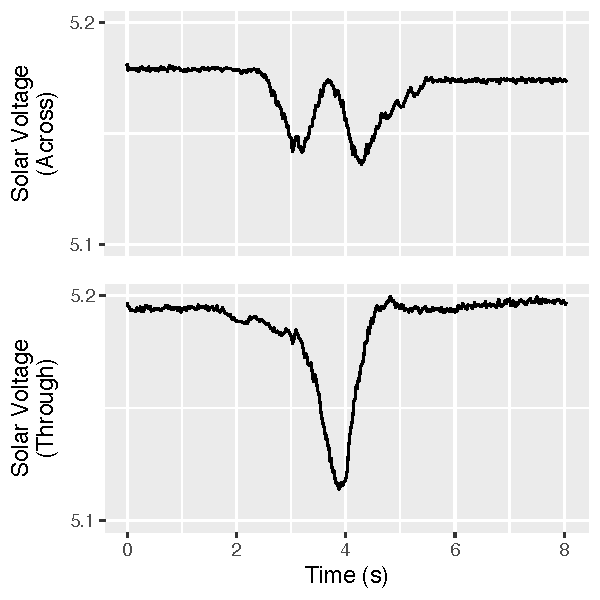
\includegraphics[width=\columnwidth]{figs/spotlight.pdf}
        \caption{These traces show the solar panel output in the presence of the ``Spotlight'' effect. The top figure shows the response when someone walks \textit{across} the ``Spotlight'', while the bottom one shows the response when someone walks \textit{through} the door.}
        \label{fig:spotlight}
    \end{subfigure}%
    %
    \hspace{30pt}
    \begin{subfigure}[t]{0.35\textwidth}
        \centering
        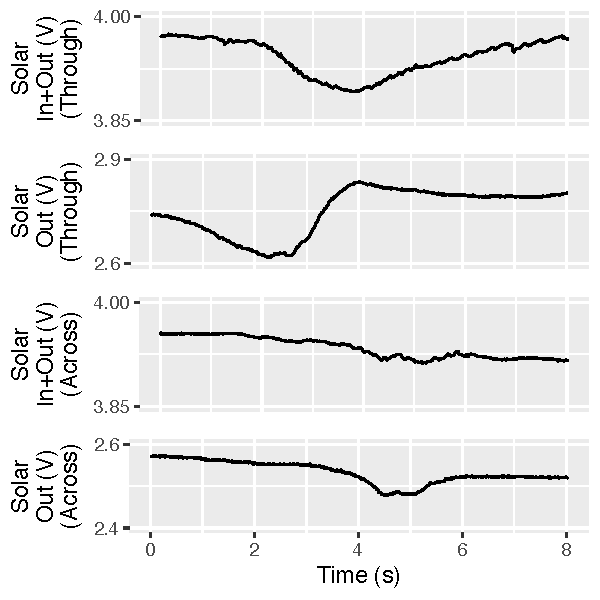
\includegraphics[width=\columnwidth]{figs/acrossAndLinger.pdf}
        \caption{ This figure compares a person walking \textit{through} the doorway (top two traces) versus walking \textit{across or by} the doorway on the outside. There is a clear delay between the two solar panel channels when someone walks through, whereas the change is reflected simultaneously when someone walks by.}
        \label{fig:across}
    \end{subfigure}
    \caption{Factors affecting \sysname operation. \label{fig:confounds}}
\end{figure*}


\paragraph{Multiple people:}
\secref{sec:normal_operation} showed the ability of \sysname to detect individual people walking through.
A practical consideration would be to examine the performance of \sysname when multiple people walk through.

In order to evaluate this, we tested two subjects walking through doorway \#1 with varying time delays between them.
This gave us control over the time separation between two events, and allowed us to examine how closely can two people walk in without being detected as one, quite large person.
We discovered that as long as two people have at least \minSeparation between them, \sysname can accurately distinguish between them, but may incorrectly classify the direction.
This limitation is introduced due to the time required by the solar panels to reset or stabilize before the next event can occur.
A subsequent logical conclusion is that if two people walk side-by-side, \ie with zero separation between them, out current prototype is unable to detect them as two events.

\paragraph{The ``Spotlight'' effect:}
An interesting consequence of light-based detection is a problematic condition that can occur especially in mixed-light settings, when an intense low-angle light source dominates the illumination.
This effect appears in the presence of a very focused source of light that dominates the illumination around the doorway, such as a spotlight or a west-facing window in late evening when the sun blazes directly through.
When someone walks across the light source, even if they are far from the doorway, it can be detected falsely by \sysname as someone walking through.
\sysname detects people based on a decrease in the harvested energy and momentarily blocking the spotlight can produce a significant decrease in voltage on both solar channels.
Interestingly, we can see from \figref{fig:spotlight} that the raw output of the solar panels look sufficiently different for someone walking \textit{across} the focused source as compared to when someone walks \textit{through} the doorway in presence of a focused source.
%At present, \sysname is equipped to detect events with good accuracy.
With further signal processing, \sysname could distinguish these spotlight events so that such events would not cause false triggers.


\paragraph{Detection Range/Walking across, not through:}
\label{subsubsec:range}
Considering that \sysname uses the blocking of light to detect a person, there will be an influence radius inside which a person starts affecting the sensor.
If someone walks by either side of a doorway monitored by the \sysname sensor and are within the radius, they will trigger the detector circuits and register as an event by \sysname.
We ran an experiment to determine this radius of influence where the subject was directed to walk by on either side of the doorway at increasing distances from the sensor.
We started with a distance of 30 cm (~1 foot) and went up to 152 cm (~5 feet), in increments of 30 cm (~1 foot).
For each distance, we asked the subject to walk by multiple times and recorded how many false triggers were detected.
An example of this is shown in \figref{fig:across}.
We have observed that under typically indoor lighting conditions for distances greater than 91 cm away from the doorway, there is a negligible chance of triggering false events.

It is interesting to note from \figref{fig:across} that there is a distinguishable difference between this event as compared to someone walking through the doorway.
Since they are walking only on one side of the doorway, their effect on both channels is not delayed by the angling of the solar panels, as is the case with walking through.
As with the ``Spotlight'' effect, we should be able to extract this difference with further signal processing and learning. %and we attempted a stab at addressing this confounding condition further in the uncontrolled experiments that will be discussed later.  %\fxnote{[This might need some rewording for the fact that we do try to handle this in the uncontrolled experiments.-NT]}

\paragraph{Lingering in the doorway:}
Another situation that causes false triggers is when a person approaches the doorway, but simply pokes their head in.
Upon evaluation, we discovered that as long as the person is poking their head in the doorway, the solar panel output remains at a lower level, and when they exit, it rises back again.
Although the current system implementation isn't equipped to differentiate between someone passing through and someone lingering in doorway, there is a clear difference in the raw waveform outputted by the solar panel.
This case is similar to \secref{subsubsec:range} in terms of being distinguishable from a person walking through and with some careful, direct signal processing it is definitely possible to differentiate between the actual and the confounding case.

\subsubsection{Microbenchmarks}
\label{sec:microbenchmarks}
The more effective \sysname is at maintaining a low-power state when idling, the more available \sysname is for detecting doorway events and monitoring occupancy.
The energy requirements for detection and active computation must be kept low as well.
Unlike intermittent computing systems, \sysname must intentionally avoid power failures.
We measured the current draw of our \sysname prototype while it was mounted on doorway \#1.
The idle draw of the system was \SI{7}{\micro\ampere}, showing that \sysname can survive in a doorway with minimal light and energy harvesting.
We gathered other benchmarks of system energy performance in each of sysname's different operating modes. To seperate harvesting and consumption, these measurements were made after the MIC841 hysteresis chip. So, the actual power and energy is slightly higher (by \SI{1.5}{\micro\ampere} according to the datasheet).


% Idle Current: 7-11uA, MCU not active
% Timer / ISR handling, single detector, no event : 190-230us, MCU active
% Doorway Event, MCU active, compute time: 7.2ms
%
% Peak current for active: 500uA
% Avg current for active: 220uA
% 2.8V
\begin{table*}[t]
\footnotesize
\begin{tabular}{@{}p{1.4in}llc@{}}
\toprule
\textbf{State}          & \multicolumn{1}{r}{\textbf{Avg. Current}} & \multicolumn{1}{r}{\textbf{Peak Current}} & \multicolumn{1}{r}{\textbf{MCU Active}} \\ \midrule
\textit{Waiting (Sleep Mode)}       	& \SI{7}{\micro\ampere}	&  \SI{11}{\micro\ampere}	& \textcolor{magenta}{\xmark} \\
\textit{Maintenance Actions} & \SI{200}{\micro\ampere}	& \SI{250}{\micro\ampere}		 & \textcolor{green}{\cmark} \\
\textit{Doorway Event Handler} & \SI{500}{\micro\ampere}	& \SI{700}{\micro\ampere}	    & \textcolor{green}{\cmark} \\ \midrule
\end{tabular}
\caption{Microbenchmarks for \sysname current consumption.}
\label{tab:microbenchmarks}
\end{table*}


Since \sysname is event-driven, its actual power consumption varies depending on the activity underneath the sensor. As shown in \tabref{tab:microbenchmarks} the idle power draw of \sysname is low (\SI{7}{\micro\ampere}). When timers or detector circuits trigger interrupts (maintenance events) the system draws \SI{440}{\micro\watt} for a few \si{\micro\second}.
Computing walking direction, storing data, and transmitting results when an event ends is more expensive~(\SI{1100}{\micro\watt}, on average).
During typical operation, these higher-power events account for an insignificant fraction of the device's runtime, and the average power draw is often indistinguishable from the idle draw.
Overall the energy consumption of the system is low, but could be further improved with careful tuning of resistance values, sleep states, and the analog circuitry.







\subsection{\sysnames in the Wild}


\begin{figure}[t]
\centering
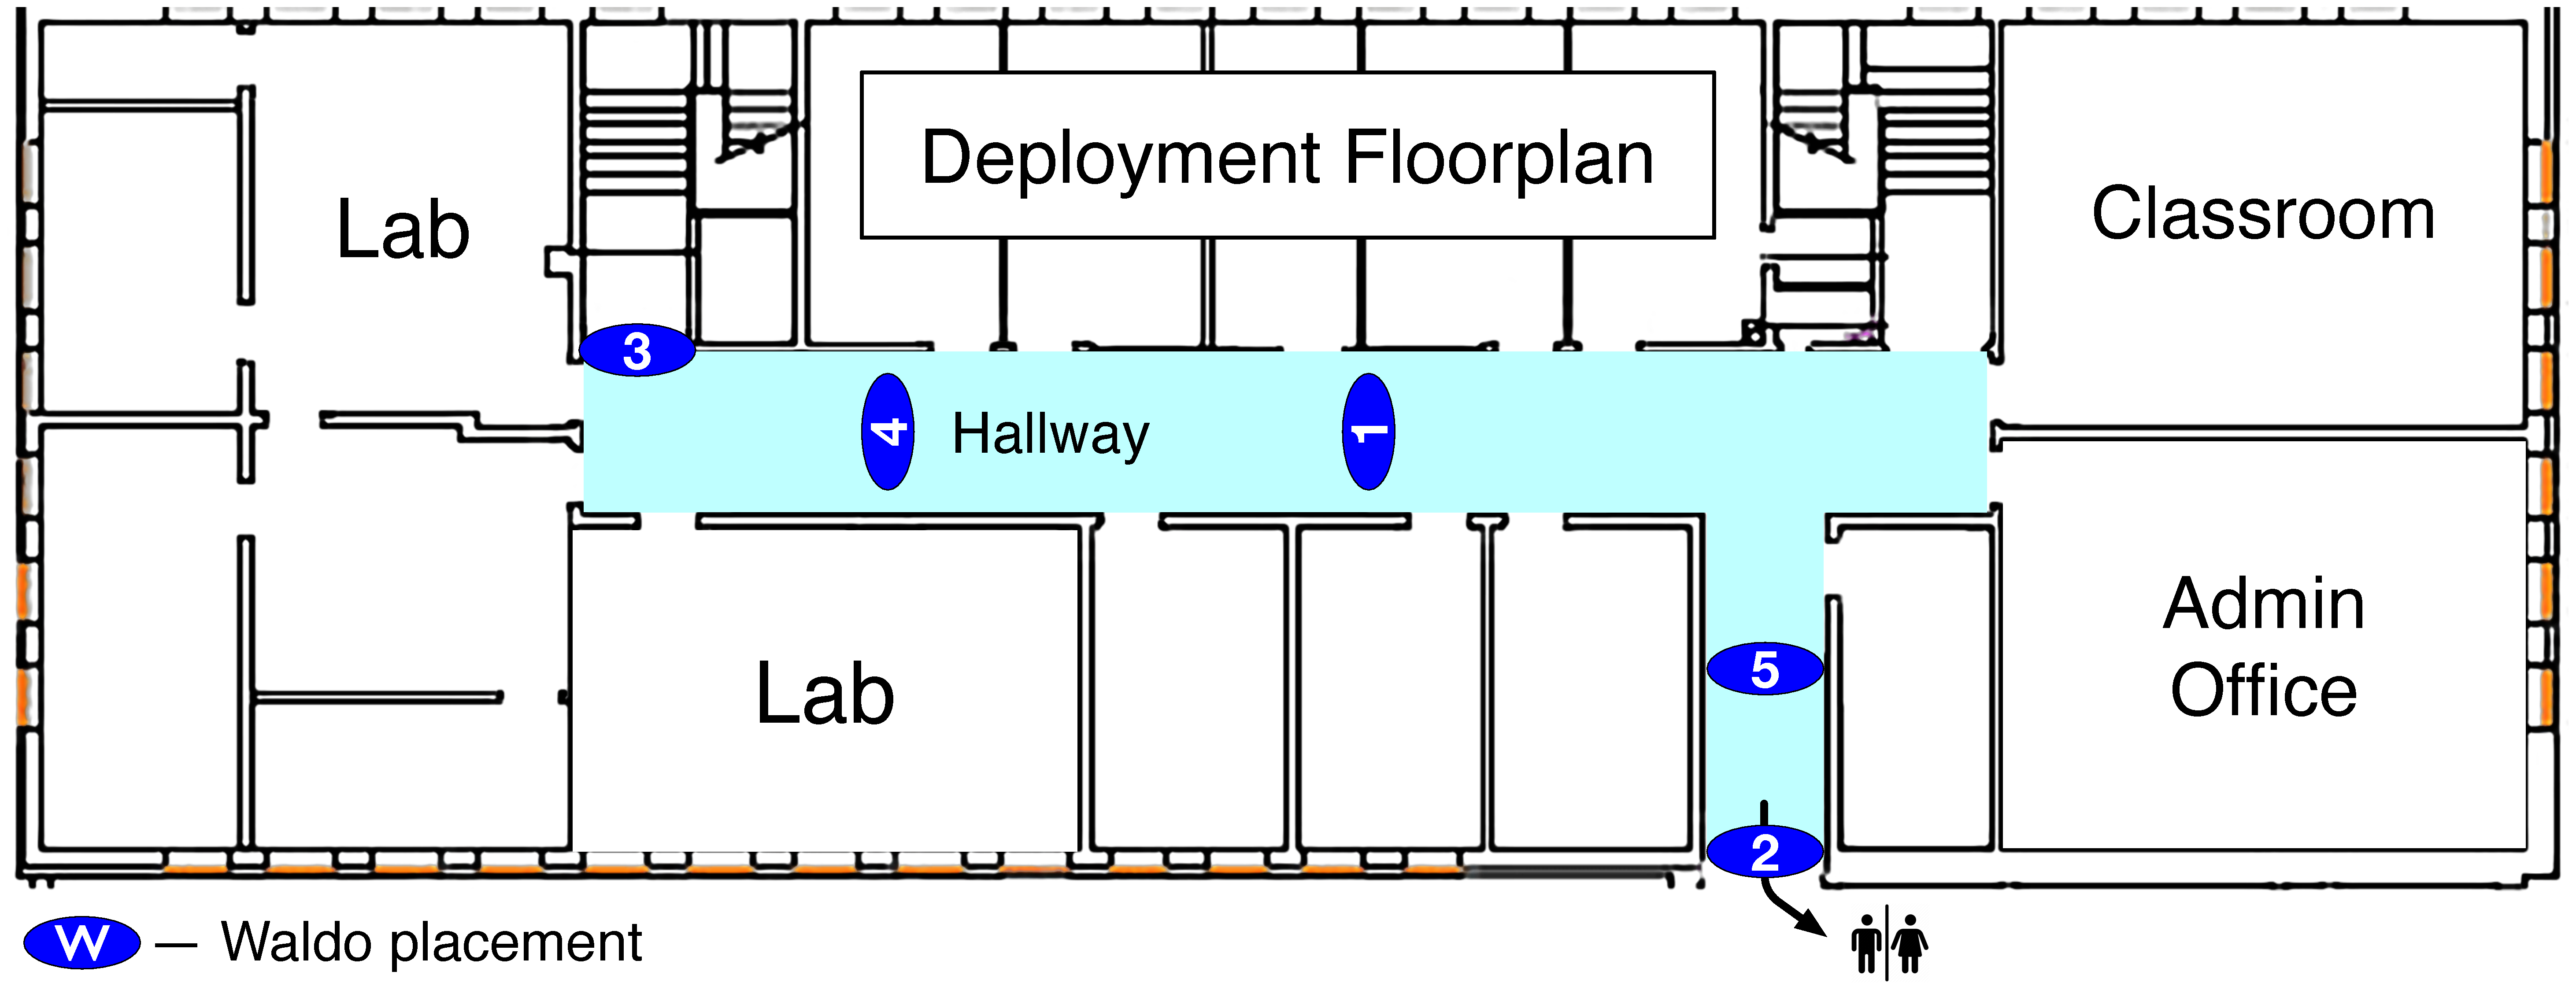
\includegraphics[width=0.8\columnwidth]{figs/floorplan.pdf}
\caption{\sysname deployment locations for the in-the-wild experiments. Each location features different lighting conditions as well as traffic patterns resulting from the adjoining labs, offices, and classrooms. \label{fig:floorplan}}
\end{figure}

%setup

In order to understand how \sysname behaves in uncontrolled conditions, we deployed multiple \sysname units along a hallway that connects offices, labs, classrooms, and bathrooms at locations shown in \figref{fig:floorplan} for a collective total of \ITWdays.  


\subsubsection{Experimental Setup.}

\begin{table*}[t]
\footnotesize
	%\begin{tabular}{@{}p{0.65in}>{\centering\arraybackslash}p{0.4in}>{\centering\arraybackslash}p{0.4in}p{0.4in}p{0.4in}p{1.1in}p{0.55in}p{0.55in}p{0.8in}p{0.55in}@{}}
	\begin{tabular}{@{}p{1.0in}p{0.2in}llp{0.2in}p{0.6in}p{1.3in}p{0.6in}l@{}}
	\toprule
	\multirow{2}{*}{\textbf{Location}}	&	\multicolumn{4}{c}{\textbf{Dimensions (cm)}} & \multirow{2}{*}{\textbf{Lighting}} & \multirow{2}{*}{\textbf{Traffic Profile}} & \textbf{Days}& \textbf{Ground Truth}  \\
		& & Height & Width 	&  						&	&  &   \textbf{Deployed} & \textbf{Events} \\\midrule
	W1 & & 243 & 235  & & Indoor  & Light/Moderate   & 17    & 436   \\ %Hallway1
	W2 & & 221 & 180 & & Indoor  & Light/Moderate    & 18   & 923  \\ %Hallway2
	W3 & & 202 & 149 & & Mixed   & Moderate/High/Bursts& 10 & 1067  \\	%Stairs
    	W4 & & 236 & 241  & & Indoor  & Moderate/High/Bursts & 10& 1070 \\ %LabHW
	W5 & & 239 & 190 & & Indoor  & Moderate/High/Bursts  & 9& 1294  \\ %preHW2
	\bottomrule
	\end{tabular}
	\caption{In-the-Wild deployment location descriptions and counts of ground truth events over the days deployed.
	\vspace{1mm}
	\label{tab:ITWcategoryfreq}}

\end{table*}

We conducted in-the-wild experiments in two sessions. In the first, sensors were deployed at two locations (W1 \& W2) for 24 days at the end of an academic semester and into the holiday class break.
We observed events on 18 of the days (only 17 for one of the sensors). 
In the second session, we deployed at three different locations (W3--W5) for an additional 11 days, with events recorded on only 9--10 days. This second session, at the start of a new semester, had heavier traffic, as shown in \tabref{tab:ITWcategoryfreq}.
The locations differed in light levels, width, and height, while providing a range of lighting and behavioral conditions. 
For example, the sensors near a classroom encounter multiple confounding cases like lingering and crowds passing under a doorway, while the ones near a lab or office are affected by lingering, spotlights, and occasionally crowds.
We selected hallways in order to observe a wider range of natural traffic patterns, including multiple people walking together under the sensors. 
At each location, we installed a \sysname sensor, a commercial ceiling-mounted EnOcean occupancy sensor~\cite{EnOcean}, and a camera to provide a ground truth confirmation of hallway activities. %Dimensions for these locations are reported in \tabref{tab:ITWresults}.  %The lab doorway is 34.5" x 79.5" and the light level is 86 lux inside the room and 91 lux outside of the room. The classroom doorway is 35" x 87" and the light level is 91 lux inside the room and 100 lux out of the room. The hallway is 76" x 93" and the light level on one side of \sysname is 94 lux and 89 lux on the other side. 
All locations have tile flooring on both sides of the sensors and are typically well enough lit to transmit a packet once after at least 30 seconds have passed.  This is usually ample time for the system to send a packet for every five detected doorway events or heartbeat (nothing has happened in two-minute) events, as events take at least 6 seconds each to process. 
%\hey{I find it a bit awkward to define this in terms of number of doorway events. Since event rate can very wildly. Can we instead relate this to time?} 
We also deployed wall-powered basestations to collect the transmitted data from the batteryless \sysname devices and EnOcean sensors.
Each basestation is an Internet-connected Raspberry Pi with a CC1101 radio and an EnOcean receiver that receives packets and stores them in an SQL database for later retrieval. 
We deployed two base stations for redundancy---one would have been sufficient.   

At each instrumented passageway, we also place a video camera that continuously collects ground truth information by recording the actual doorway events. 
We manually labeled all recorded events by watching the videos and annotating by storing the time and a description of each event---\textit{in, out, pass-by}, as well as more complex cases like lingering, people changing direction under the sensor (u-turns) and multiple people passing in or out in a group. 
In order to make sense of the wide range of observed behaviors, we sorted the events into 3 different categories: simple events, multiple-people events, and complex events. 
Simple events include simple ins, outs, and very close pass-by events with only one person around the sensor within a 6-second window of time.
Multiple people events involve multiple people that pass under the sensor going in the same direction within a 6-second window.  
These events range from 2 people walking side-by-side or close succession to 23 people all exiting at the same time when classes let out.
All other events fall in the complex category, including lingering, changing directions underneath the sensor, and multiple people going in different directions under the sensor.  

We compare these ground truth events against the sequence of events \sysname detects.
\sysname send a message to the basestation once it records at least five events or heartbeats and has enough harvested energy.
\sysname generates heartbeat events after two minutes of inactivity. 
So, during long periods of inactivity, \sysname will generate and send a packet every 10 minutes (consisting of 5 heartbeats) to let us know that it is still alive and has not seen any new events. 
This heartbeat frequency was selected for this experiment to help us distinguish between periods of inactivity (no detected events), dropped packets, and system failures.
This frequency can also be adjusted to balance these liveness concerns with energy budget constraints.

\begin{figure}[t]
\centering
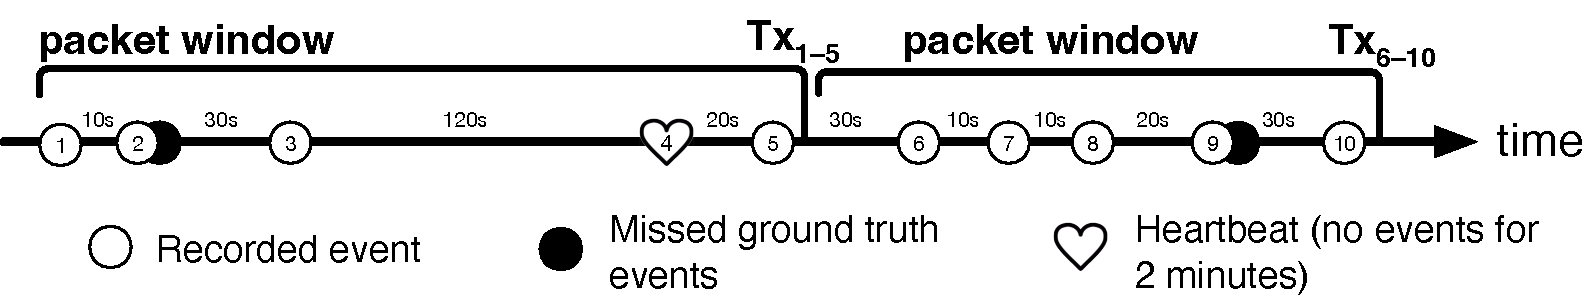
\includegraphics[width=0.9\columnwidth]{figs/timeline.pdf}
\caption{ The ground truth event timeline of our in-the-wild deployment and how it is divided into packet windows based on the when the packet is recieved immediately after processing the fifth event record within the packet window. The heart at event 4 represents a heartbeat event generated by \sysname when there have been no detected events for 2 minutes.  The two examples of recorded event and missed ground truth events represent where two individuals walk through in quick succession, such that the sensor only identifies them as one event.  This example provides a high-level view of how we compute the event statistics within a window.  \label{fig:eventtimeline}}
\end{figure}

Each network packet that \sysname sends includes the sequence of the events and heartbeats, an estimate of time that has past between each event, their classifications, and a CRC computed over the recorded values to protect against packet corruption. 
As a simple redundancy mechanism in case of packet loss, each radio transmission includes the last two previously-sent packets along with the current packet. 

For simplicity, \sysname currently has no sense of absolute time---just relative inter-event time.
In order to reconstruct the sequence of events, the time the basestation received the packet is used as a reference to match windows of events to the ground truth data.
This time is closely correlated to the time of the packet's last event.
So, we use these times to match ground truth events with the events recorded by the \sysname sensors.

%Looking at high level detection of events
\subsubsection{Data Collection and Analysis Method.}
Each packet encodes the sequence of 5 events or heartbeats that \sysname recorded and an estimate of time that has past since the last event or heartbeat recorded.
A packet received at the basestation is matched with a series of ground truth events based on the packet's receive time, the estimated inter-event times, and the duration of \sysname's event window (\SI{6}{\second}).  
This helps account for minor human errors in labeling event times, as it is not always clear exactly when someone started affecting the sensor from video data.
If two ground truth events match a packet, the one closest (in time) is chosen and mapped to the 5th event associated with this packet.
Using the information stored in the packets about number of events and their estimated associated time between the events, we can estimate the match of the other ground truth events with their likely corresponding records in the packet record sequence to analyze hits or misses and if the classified direction was correct.  
\figref{fig:eventtimeline} shows a high-level example of the how ground truth events are divided by the packet window based on the received time of the packet in order to calculate correctly detected events and possible missed events, as well as when detected, if they were correctly classified. 
Each \sysname packet has a monotonically increasing packet ID, which we use to detect packet losses.
If a packet is dropped or corrupted, it can be reclaimed from the following transmission, which includes the last two packets sent. 
%We tossed out activity that was only seen on the very edge camera's video (like a shadow from activity out of camera view) but was likely out of the range of our sensor. 
	
%Packets that map to a ground truth event are considered \textit{confirmed packets}.
%All other packets that could not be mapped to an event (within 30s), are still valid packets that represent five events that \sysname detected and must be considered. 
%We insert these packets into the event sequence and mark them as \textit{false positive} packets.
%The false positive packets may still contain valid data associated with the ground truth.
%The fifth event that generated the packet may have just been missed in the ground truth. 
%These confirmed and false positive markers divide up the ground truth data into probable event windows in order to make a meaningful comparison with the packet summaries.
%We then gather statistics on the number of probable events associated with each packet. 
%Confirmed packets are included in the associated window counts, however, false positive packets, while still providing a meaningful anchor for the probable event window, did not have an event closely associated enough to add to the probable event window counts.  

%We reason about the number of events that \sysname actually detects in these ground-truth based probable event windows by drawing on two characteristics of the system design. 
%One, each packet encodes five events, and two, every packet will have a different packet id number, one greater than the last packet.
%Using this knowledge, we can figure out which packets, if any, we missed (what packet id numbers were absent on the basestation?) and how well \sysname \textit{detected events}, even if it may have classified events incorrectly.
%When all the ground-truth events in the event window were explained by the number of events in the anchor packet and missed packets, we considered the window to be accounted for. 
%When they are not, we know that either events were recorded (on video) but not detected by \sysname, denoted as \emph{misses}, or \sysname detected more events than were reported in the ground-truth data, which we called extras. 
%\figref{fig:eventtimeline} shows a high level example of the how ground truth events are divided by the anchor packet time in order to calculate correctly identified event, incorrectly identified events and misses. 
%These values are aggregated over all packet windows in the ground truth data. \hey{I don't understand what this paragraph is saying. Remove? update?}


\begin{table*}[t]
	\footnotesize
		\begin{tabular}{@{}p{0.9in}p{0.8in}lllp{0.12in}p{0.2in}llp{0.2in}ccc@{}}
		%\begin{tabular}{@{}p{0.45in}>{\centering\arraybackslash}p{0.6in}>{\centering\arraybackslash}p{1in}p{0.4in}p{0.6in}p{0.35in}p{0.35in}p{0.25in}p{}p{}p{}@{}}
		\toprule
		\multirow{2}{*}{\textbf{Location}} & \textbf{Ground Truth} & \multicolumn{3}{c}{\textbf{Frequency of Events by Type}} & &\multicolumn{4}{c}{\textbf{Simple Events}} & \multicolumn{3}{c}{\textbf{Accuracy}} \\
	 & \textbf{Events} & Simple & Multi-Person*   & Complex   & &  & In  & Out  &  & In        & Out      & Total        \\  
	\midrule
	W1   & 436   & 91\%   & 4\%    & 5\%  & & & 201   & 190  &  & 71\%   & 96\%    & 83.12\%                   \\ %Hallway1. 91 is really 91.5 so 92 but then they dont add to 100
	W2   & 923   & 89\%   & 4\%    & 7\%  & & & 426   & 388  &  & 99\%   & 77\%    & 88.82\%                   \\ %Hallway2
	W3   & 1067  & 83\%   & 14\%   & 3\%  & & & 505   & 291  &  & 91\%   & 88\%    & 90.32\%                   \\ %Stairs
	W4   & 1070  & 83\%   & 14\%   & 3\%  & & & 343   & 503  &  & 92\%   & 98\%    & 95.51\%                   \\ %LabHW
	W5   & 1294  & 85\%   & 10\%   & 5\%  & & & 579   & 512  &  & 97\%   & 93\%    & 94.96\%                   \\ %preHW2
		\bottomrule
		\end{tabular}
		\caption{Waldo in-the-wild deployment frequency of events by type at each deployment location and accuracy on how the system performed on classifying the simple ins and outs that were encountered over the deployment.
		\vspace{1mm}
		\\\textsuperscript{*}Multi-Person Events --- This category of events represents only multiple persons traveling under the sensor going in the same direction.
		\label{tab:ITWresults}}
	
	\end{table*}
	


\subsubsection{Results.}  
%break down by category
\sysname performed well when detecting activity that was taking place under the sensor and, when the activity was close enough, around the sensor.
All events that happened under the sensor were detected, and throughout the deployment, we lost only one packet due to transmission errors. 
Based on the previous and subsequent packet numbers, we know the sensor recorded something but we can not verify whether the one ground truth event that occurred during this time was detected correctly.
\tabref{tab:ITWresults} shows the frequency of the different event categories that the sensors experienced while deployed and \sysname's accuracy on classifying the simple in and out events where a single user walked under the sensor.

\textbf{Simple Events} significantly outnumbered the other two event categories across all sensor locations.
\sysname is specifically designed to detect simple one-person ins and outs, and these are the most common form of traffic we observed.
\sysname detected all of the simple events, and correctly classified their direction 83--95.5\% of the time, depending on the sensor location.
Nearly all misclassified simple events were misclassified as pass-by events, though a few out events were misclassified as in events. 

As mentioned before, only one of the deployment locations~(W4) was used for both gathering training data and our in-the-wild deployment.
While this location (unsurprisingly) outperformed the others, the others were close behind---indicating both that the trained model was able to work well when used in different lighting conditions and that future \sysname iterations might achieve small performance improvements by adapting the model in situ based on observed light conditions. 


\sysname also detected the \textbf{Multi-Person} and \textbf{Complex} events, including lingers, u-turns, and multiple people affecting the sensor in quick succession; however, the sensor was not always able to accurately estimate number of people passing by or their direction.

\textbf{Multi-Person Events}---multiple people pass together or in quick succession under the sensor in the same direction---typically result in undercounting. 
When the events completed within \sysname's \SI{6}{\second} event window---common when two people were walking side-by-side---the events were reported as an in event or an out event, and the event directions were nearly always classified accurately (comparable to the accuracies reported for the simple events).
%
When these events lasted longer than \SI{6}{\second}, \sysname reported a group of multiple consecutive events, with the first event usually classifying the event direction correctly and subsequent events often misclassified when \sysname's event windows often captured partial events.

\textbf{Complex Events}, including lingers, u-turns, near pass-bys, and multiple people passing the sensor simultaneously in opposite directions behaved similarly, producing a group of one or more consecutive events, except that the direction estimate for the first event in the group is also often incorrect.
Another key difference is that some complex events can result in overcounting.
For example, a single person lingering under a \sysname sensor for a few minutes will produce multiple consecutive events.
The longer the person spent underneath the sensor, the more of these events \sysname would record.


Both Multi-Person and Complex events represent confounding cases for \sysname---and challenging cases for technologies for monitoring human movement through buildings.
While we plan to address them in future improvements (\secref{sec:discussion}), for now their impact depends on traffic conditions.
Under usual passageway conditions, a user wanting to count people can treat isolated events (events with more than a \SI{6}{\second} gap between them) as single person events with reliable direction estimates and end up with slight underestimates.
Sequences of consecutive events (with no gap) can, for now, be treated as reliable activity measurements but not accurate people counts or direction estimates.


The first phase of our deployment (W1 \& W2), during end-of-semester traffic conditions, saw fewer groups moving together and less overall traffic, and 89--91\% of the observed events were simple in and out events with 9--11\% confounding events (mostly two-person side-by-side events and some lingers).
As traffic increased at the start of the following semester, locations W3--W5 saw an increase in overall traffic and confounding events increased to 15--17\% of the total events.
In spite of the traffic increase, both phases were dominated by simple events, and \sysname provided information suitable for accurate people counting.
Of course, in some extremely high traffic areas (e.g., the entrance to a sporting event or concert) we expect that \sysname would have a high number of confounding events and behave like an activity sensor providing less information about individual people and their direction.  


\subsubsection{Commercial Sensor Comparison}
\label{sec:enocean}
%We note that it is difficult to fairly compare the performance of different occupancy-monitoring systems except in their accuracy. For example, CeilingSee~\cite{yang2017ceilingsee} uses 16 devices to instrument a room, while \sysname and SonicDoor~\cite{sonicdoor-buildsys2017} place one device in the doorway, and AURES~\cite{shih2016aures} places a single device in the middle of a room. 
%For this reason, we investigate the accuracy of \sysname against our manually gathered ground truth (visually verifying a person entering or exiting the room) instead of comparing to another occupancy-detection system.
As mentioned earlier, in order to compare \sysname to its closest commercially available alternative, we deployed a batteryless commercial ceiling-mounted PIR occupancy sensor by EnOcean~\cite{EnOcean} alongside our \sysname sensors on each passageway. While other similar sensors are available, we selected the EnOcean sensor because it was actually a battery-free commercial option that did not use rechargeable batteries and had transparent product specifications easily available online.  This sensor also was more programmable for expermental repeatability and, at the time of purchase, more easily available in our country.
This sensor is the powered by harvested energy, and uses ambient light~(IR) changes to detect movement.
Unlike \sysname, this sensor only detects activity/occupancy (but no direction information).


EnOcean sensors send two types of packets: an \emph{occupied packet} when an event is detected and an \emph{unoccupied packet} after 10 minutes of inactivity has passed followed by every 30~minutes after that.  
If movement is detected, it sends an occupied packet to a receiver attached to the same basestation we use to receive packets from \sysname.
Like before, the basestation collects these packets and stores them in an SQL database for later processing and comparison with the ground truth data.
Once EnOcean detects an event and sends an occupied packet, it will not detect any more events for the next 2~minutes. 
While this 2~minute blind-spot allows the device to recharge between radio transmissions, it is also a considerable disadvantage when compared to \sysname's 6--7~second blind-spot.
\figref{fig:enoceanVwaldo} shows how the two sensors behaved in the face of a simple event and in the presence of slightly higher traffic during our deployment.


We use the data from both sensors to estimate the number of people that walk through the passageway, as shown in~\tabref{tab:ITWEnOceanVWaldoresults}.
With its smaller blindspot, \sysname outperforms the EnOcean sensors in all cases, but especially during our second deployment~(W3--W5) with increased traffic and more multi-person events.
When profiling traffic through passageways, \sysname not only provides higher resolution information, but it also provides additional direction information to building managers looking to accurately estimate traffic flows.

\begin{figure}[t]
\centering
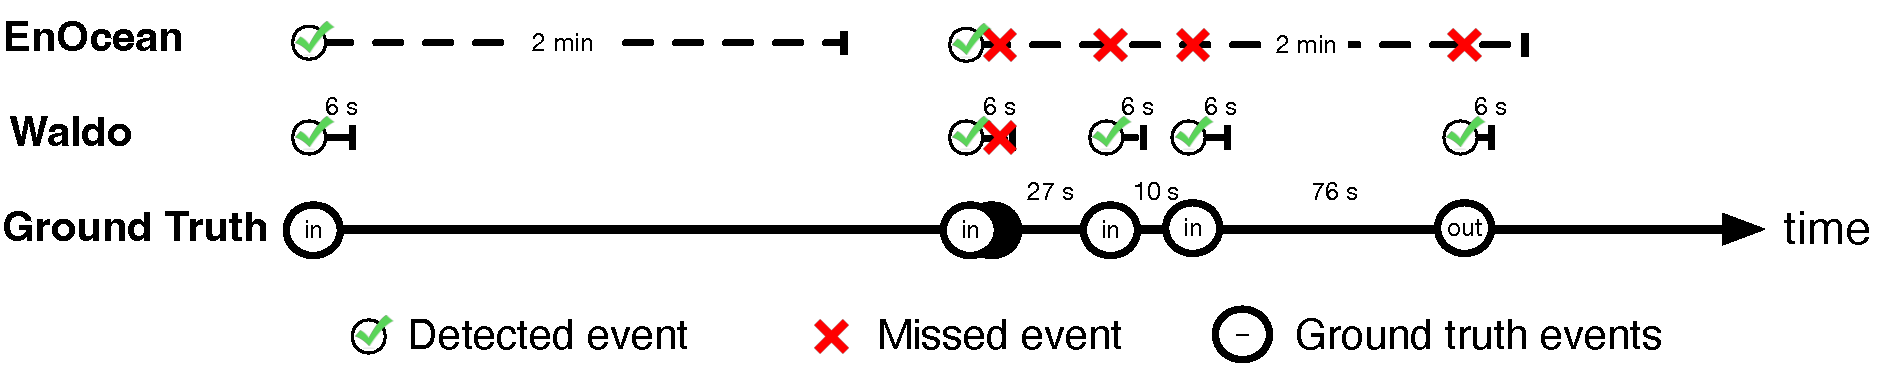
\includegraphics[width=0.9\columnwidth]{figs/enocean_v_waldo_v_gt.pdf}
\caption{ The ground truth event timeline of our in-the-wild deployment and how \sysname and EnOcean sensors detect a sequence of events.  This example provides a high level view of each systems detection accuracy and is based on actual data collected from our in-the-wild experiments.  \label{fig:enoceanVwaldo}}
\end{figure}

\begin{table*}[t]
\footnotesize
	\begin{tabular}{@{}p{1.0in}p{0.9in}p{0.8in}p{0.7in}p{0.7in}p{0.5in}@{}}
	\toprule
	\multirow{2}{*}{\textbf{Location}}	&	\textbf{Gnd Truth} & \textbf{\sysname} & \textbf{\sysname} & \textbf{EnOcean} 	& \textbf{EnOcean}	\\
	& \textbf{Total People} & \textbf{Detected} & \textbf{Accuracy} &  \textbf{Detected} & \textbf{Accuracy} \\\midrule
	W1 & 452 & 434 & 96\% & 304 & 67\% \\ %Hallway1
	W2 & 961 & 925 & 96\% & 613 & 64\% \\ %Hallway2
	W3 & 422 & 308 & 73\% & 174 & 41\% \\	%Stairs
        W4 & 1440 & 1107 & 77\% & 551 & 38\% \\ %LabHW
	W5 & 1637 & 1316 & 80\% & 640 & 39\% \\ %preHW2
	\bottomrule
	\end{tabular}
	\caption{Comparison of performance between the EnOcean and Waldo sensors at each location during the in-the-wild deployment.  This comparison show how well each system was able to detect and monitor the number of people moving through a passageway.  Due to high traffic and burst conditions that occur when class lets out, both systems are affected with being able to detect number of people passing through the passageway as EnOcean has a 2-minute blind spot after the first event is detected and Waldo has a 6 second event window where it is processing a single event and misses multiple people traveling within that event window.
	\vspace{1mm}
	\label{tab:ITWEnOceanVWaldoresults}}

\end{table*}

%setup



%\subsubsection{Discussion of In-Wild Results.}
%These results are impacted by people lingering by doorways, entering or exiting in crowds, making abrupt changes in direction under the sensor, and by individuals changing out cameras to collect ground truth or preforming basic system maintenance.  The matched windows to draw our comparison was impacted by sporadic camera malfunctions which limited available ground truth, collection over spring break which dampened overall user activity for several days, and a school wide power-outage for system maintenance which impacted the available light to the sensors as well as the power for the basestations to collect data and log them to the SQL database.


%\fxnote{[ I created  confusion matrix using R based on the collected data, but that data needs some cleaning like i+o, (i+)o in the %detected direction-AA]}
%section:  System Accuracy
	%just walking through
		%-just using interrupts
		%-just detection circuits
		%hw detection only vs sw enhancements
	%detecting direction
		%-just using interrupts
		%-just detection circuits
		%hw detection only vs sw enhancements
%if we get to sw at all





%section:  extreme cases (how low can we make lighting and system still work)?
